\documentclass[]{article}
\usepackage[margin=2cm]{geometry}

%opening
\title{Exercises Set: Calculus\\ \large Solutions}
\author{DSBA Mathematics Refresher 2026}
\date{}

\usepackage{amsmath}
\usepackage{amsfonts}
\usepackage{amsthm}
\usepackage{amssymb}
\usepackage{mathrsfs}
\usepackage{stmaryrd}
\usepackage{tikz}

\newcommand{\Q}{\mathbb{Q}}
\newcommand{\N}{\mathbb{N}}
\newcommand{\Z}{\mathbb{Z}}
\newcommand{\R}{\mathbb{R}}
\newcommand{\Primes}{\mathbb{P}}
\newcommand{\st}{\text{ s.t. }}
\newcommand{\txtand}{\text{ and }}
\newcommand{\txtor}{\text{ or }}
\newcommand{\lxor}{\veebar}


\begin{document}

	\maketitle

	\section{Fundamental Theorem of Calculus}

	\paragraph{Generalization / Corollary}\mbox{}\\
	Let $F$ be the particular anti-derivative $F(x) = \int_0^x f(t)\,dt$.
	Using the Chasles relation $\int_0^b = \int_0^a + \int_a^b$:
	$$
	F(b) - F(a) = \int_0^b f(t)\,dt - \int_0^a f(t)\,dt
	= \left( \int_0^a f(t)\,dt + \int_a^b f(t)\,dt \right) - \int_0^a f(t)\,dt
	= \int_a^b f(t)\,dt
	$$

	This proves the result for \textit{that} anti-derivative.
	It holds in fact for \textbf{any} anti-derivative $G$ of $f$: two anti-derivatives of the same function differ by a constant, so $G = F + C$, and the constant cancels in the difference:
	$$
	G(b) - G(a) = \left( F(b) + C \right) - \left( F(a) + C \right) = F(b) - F(a) = \int_a^b f(t)\,dt
	$$
	This is why we may pick whichever anti-derivative is most convenient, and why the constant of integration is irrelevant for \textit{definite} integrals.

	\begin{center}
		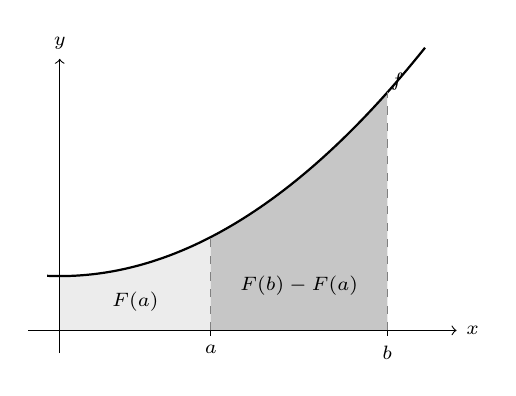
\begin{tikzpicture}[xscale=1.6,yscale=1.15]
			\fill[gray!15] (0,0) -- plot[domain=0:1.2,samples=50,smooth] ({\x},{0.3*\x*\x+0.6}) -- (1.2,0) -- cycle;
			\fill[gray!45] (1.2,0) -- plot[domain=1.2:2.6,samples=50,smooth] ({\x},{0.3*\x*\x+0.6}) -- (2.6,0) -- cycle;
			\draw[->] (-0.25,0) -- (3.15,0) node[right] {\scriptsize $x$};
			\draw[->] (0,-0.25) -- (0,3.0) node[above] {\scriptsize $y$};
			\draw[thick,domain=-0.1:2.9,samples=60,smooth] plot ({\x},{0.3*\x*\x+0.6});
			\draw (1.2,0.06) -- (1.2,-0.06) node[below] {\scriptsize $a$};
			\draw (2.6,0.06) -- (2.6,-0.06) node[below] {\scriptsize $b$};
			\draw[dashed,gray] (1.2,0) -- (1.2,1.032);
			\draw[dashed,gray] (2.6,0) -- (2.6,2.628);
			\node at (0.6,0.32) {\scriptsize $F(a)$};
			\node at (1.9,0.5) {\scriptsize $F(b)-F(a)$};
			\node[right] at (2.55,2.75) {\scriptsize $f$};
		\end{tikzpicture}
	\end{center}
	The light area is $\int_0^a f = F(a)$ and the dark area is $\int_a^b f$; together they make up $\int_0^b f = F(b)$.
	Subtracting the light area from the whole is exactly the statement $\int_a^b f = F(b) - F(a)$.

	\paragraph{Application}\mbox{}\\
	An anti-derivative of $\sin$ is $-\cos$, so
	$$
	\int_0^{\pi/2} \sin(x)\,dx = \Big[ -\cos(x) \Big]_0^{\pi/2} = -\underbrace{\cos\left(\tfrac{\pi}{2}\right)}_{=\,0} + \underbrace{\cos(0)}_{=\,1} = 1
	$$

	An anti-derivative of $\frac{1}{x^2} = x^{-2}$ is $-\frac{1}{x}$ (recall $\int x^n dx = \frac{x^{n+1}}{n+1}$ for $n \neq -1$, here with $n = -2$), so
	$$
	\int_1^4 \frac{1}{x^2}\,dx = \left[ -\frac{1}{x} \right]_1^4 = -\frac{1}{4} - \left(-\frac{1}{1}\right) = \frac{3}{4}
	$$

	\textit{Note:} both integrands are positive on the interval of integration, and both answers are positive --- always worth a glance.


	\section{Integration Techniques}

	\subsection*{Substitution / Change of Variable}

	\paragraph{Exercise 1:} $\displaystyle \int \frac{2x}{x^2+1}\,dx$

	Let $u = x^2 + 1$; then $\dfrac{du}{dx} = 2x$, i.e. $du = 2x\,dx$, which is exactly the numerator:
	$$
	\int \frac{2x}{x^2+1}\,dx = \int \frac{du}{u} = \ln|u| + C = \ln\left(x^2+1\right) + C
	$$
	(no absolute value is needed since $x^2 + 1 > 0$).

	\textit{Check:} $\dfrac{d}{dx}\ln(x^2+1) = \dfrac{2x}{x^2+1}$. \checkmark

	\textit{Remark:} this is the pattern $\int \frac{g'(x)}{g(x)}dx = \ln|g(x)| + C$, which is worth recognising directly.

	\paragraph{Exercise 2: (*)} $\displaystyle \int \frac{1}{\sqrt{1-x^2}}\,dx$

	Let $x = \sin(u)$, with $u \in \left(-\frac{\pi}{2}, \frac{\pi}{2}\right)$ so that the substitution is invertible; then $dx = \cos(u)\,du$ and
	$$
	\sqrt{1-x^2} = \sqrt{1 - \sin^2(u)} = \sqrt{\cos^2(u)} = \left| \cos(u) \right| = \cos(u)
	$$
	the last equality because $\cos(u) > 0$ on that interval. Therefore
	$$
	\int \frac{1}{\sqrt{1-x^2}}\,dx = \int \frac{\cos(u)}{\cos(u)}\,du = \int 1 \,du = u + C = \arcsin(x) + C
	$$

	\textit{Check:} this is the very definition of the derivative of $\arcsin$. \checkmark

	\paragraph{Exercise 3:} $\displaystyle \int \frac{1}{4+x^2}\,dx$

	Let $x = 2u$ (i.e. $u = x/2$); then $dx = 2\,du$ and $4 + x^2 = 4 + 4u^2 = 4\left(1+u^2\right)$, so
	$$
	\int \frac{1}{4+x^2}\,dx
	= \int \frac{2\,du}{4\left(1+u^2\right)}
	= \frac{1}{2} \int \frac{du}{1+u^2}
	= \frac{1}{2}\arctan(u) + C
	= \frac{1}{2}\arctan\left(\frac{x}{2}\right) + C
	$$

	\textit{Check:} $\dfrac{d}{dx}\left[\frac{1}{2}\arctan\left(\frac{x}{2}\right)\right] = \frac{1}{2}\cdot\frac{1}{1+\frac{x^2}{4}}\cdot\frac{1}{2} = \frac{1}{4+x^2}$. \checkmark

	\textit{Remark:} the point of the substitution is to bring the integral back to the standard form $\int \frac{du}{1+u^2} = \arctan(u) + C$.
	The same trick gives $\int \frac{dx}{a^2+x^2} = \frac{1}{a}\arctan\left(\frac{x}{a}\right) + C$.

	\subsection*{Integration by Parts}

	Recall the formula, which comes from integrating the product rule $(uv)' = u'v + uv'$:
	$$
	\int u \, v' = \Big[ u v \Big] - \int u' \, v
	$$
	The whole skill is choosing which factor plays the role of $u$ (the one that gets \textit{simpler} when differentiated).

	\paragraph{Exercise A:} $\displaystyle \int x \ln(x)\,dx$

	Take $u = \ln(x)$ and $v' = x$ (so $u' = \frac{1}{x}$ and $v = \frac{x^2}{2}$) --- differentiating the logarithm is what removes it:
	$$
	\int x \ln(x)\,dx
	= \frac{x^2}{2}\ln(x) - \int \frac{x^2}{2} \cdot \frac{1}{x}\,dx
	= \frac{x^2}{2}\ln(x) - \frac{1}{2}\int x \,dx
	= \frac{x^2}{2}\ln(x) - \frac{x^2}{4} + C
	$$
	that is
	$$
	\int x \ln(x)\,dx = \frac{x^2}{2}\left( \ln(x) - \frac{1}{2} \right) + C
	$$

	\textit{Check:} $\dfrac{d}{dx}\left[\frac{x^2}{2}\ln x - \frac{x^2}{4}\right] = x\ln x + \frac{x^2}{2}\cdot\frac{1}{x} - \frac{x}{2} = x \ln x$. \checkmark

	\paragraph{Exercise B:} $\displaystyle \int x^2 e^x\,dx$

	Take $u = x^2$ and $v' = e^x$: each integration by parts lowers the power of $x$ by one, so we apply it twice.
	$$
	\int x^2 e^x\,dx = x^2 e^x - \int 2x\, e^x\,dx
	$$
	and for the remaining integral, again with $u = 2x$ and $v' = e^x$:
	$$
	\int 2x\, e^x\,dx = 2x e^x - \int 2 e^x\,dx = 2x e^x - 2e^x
	$$
	Therefore
	$$
	\int x^2 e^x\,dx = x^2 e^x - 2x e^x + 2 e^x + C = e^x\left( x^2 - 2x + 2 \right) + C
	$$

	\textit{Check:} $\dfrac{d}{dx}\left[e^x(x^2-2x+2)\right] = e^x(x^2-2x+2) + e^x(2x-2) = e^x x^2$. \checkmark

	\paragraph{Exercise C: (*)} $\displaystyle \int x \cos(x)\,dx$

	Take $u = x$ and $v' = \cos(x)$ (so $u' = 1$ and $v = \sin(x)$):
	$$
	\int x \cos(x)\,dx = x \sin(x) - \int \sin(x)\,dx = x\sin(x) + \cos(x) + C
	$$

	\textit{Check:} $\dfrac{d}{dx}\left[x\sin x + \cos x\right] = \sin x + x\cos x - \sin x = x \cos x$. \checkmark

	\paragraph{Exercise D:} $\displaystyle \int e^{2x} \cos(2x)\,dx$

	Here neither factor simplifies when differentiated, so integrating by parts twice brings the \textit{original} integral back --- and we solve for it.
	Write
	$$
	I = \int e^{2x}\cos(2x)\,dx
	\qquad \text{and} \qquad
	J = \int e^{2x}\sin(2x)\,dx
	$$

	For $I$, take $u = \cos(2x)$ and $v' = e^{2x}$ (so $u' = -2\sin(2x)$ and $v = \frac{1}{2}e^{2x}$):
	$$
	I = \frac{1}{2}e^{2x}\cos(2x) - \int \frac{1}{2}e^{2x}\left(-2\sin(2x)\right)dx
	  = \frac{1}{2}e^{2x}\cos(2x) + J
	$$
	For $J$, take $u = \sin(2x)$ and $v' = e^{2x}$ (so $u' = 2\cos(2x)$):
	$$
	J = \frac{1}{2}e^{2x}\sin(2x) - \int \frac{1}{2}e^{2x} \cdot 2\cos(2x)\,dx
	  = \frac{1}{2}e^{2x}\sin(2x) - I
	$$
	Substituting the second relation into the first:
	$$
	I = \frac{1}{2}e^{2x}\cos(2x) + \frac{1}{2}e^{2x}\sin(2x) - I
	\qquad \Longrightarrow \qquad
	2I = \frac{1}{2}e^{2x}\left(\cos(2x) + \sin(2x)\right)
	$$
	so
	$$
	\int e^{2x}\cos(2x)\,dx = \frac{1}{4}e^{2x}\Big( \cos(2x) + \sin(2x) \Big) + C
	$$

	\textit{Check:} differentiating,
	$$
	\frac{1}{4}\Big[ 2e^{2x}\left(\cos 2x + \sin 2x\right) + e^{2x}\left(-2\sin 2x + 2\cos 2x\right) \Big]
	= \frac{1}{4}e^{2x} \cdot 4\cos(2x) = e^{2x}\cos(2x) \ \checkmark
	$$

	\subsection*{Further integration techniques}

	\paragraph{Exercise $\alpha$:} $\displaystyle \int \frac{3x^2-2x-1}{x^3-x^2+x-1}\,dx$

	\textit{Factor the denominator} by grouping:
	$$
	x^3 - x^2 + x - 1 = x^2(x-1) + (x-1) = (x-1)\left(x^2+1\right)
	$$
	\textit{Factor the numerator:} $x = 1$ is an obvious root ($3 - 2 - 1 = 0$), so $(x-1)$ divides it, and
	$$
	3x^2 - 2x - 1 = (x-1)(3x+1)
	$$
	The factor $(x-1)$ cancels, and for $x \neq 1$:
	$$
	\frac{3x^2-2x-1}{x^3-x^2+x-1} = \frac{3x+1}{x^2+1}
	$$
	We split this into the two standard pieces:
	$$
	\int \frac{3x+1}{x^2+1}\,dx
	= \frac{3}{2}\int \frac{2x}{x^2+1}\,dx + \int \frac{1}{x^2+1}\,dx
	= \frac{3}{2}\ln\left(x^2+1\right) + \arctan(x) + C
	$$
	valid on any interval not containing $x = 1$.

	\textit{Remark:} had the numerator been $3x^2 - 2x + 1$, it would have been \textit{exactly} the derivative of the denominator, and the answer would simply have been
	$$
	\int \frac{3x^2-2x+1}{x^3-x^2+x-1}\,dx = \ln\left| x^3-x^2+x-1 \right| + C
	$$
	Always compare the numerator with the derivative of the denominator before doing anything else.

	\paragraph{Exercise $\beta$: (*)} $\displaystyle \int_0^{+\infty} e^{-x}\,dx$

	An improper integral is \textit{defined} as a limit, so we integrate up to $a$ and then let $a \to +\infty$:
	$$
	\int_0^{+\infty} e^{-x}\,dx
	= \lim_{a \to +\infty} \int_0^{a} e^{-x}\,dx
	= \lim_{a \to +\infty} \Big[ -e^{-x} \Big]_0^{a}
	= \lim_{a \to +\infty} \left( \underbrace{-e^{-a}}_{\longrightarrow \, 0} + \underbrace{e^{0}}_{=\,1} \right)
	= 1
	$$
	The limit exists and is finite: the integral \textbf{converges}, and its value is $1$.

	\textit{Note:} the area under an unbounded region can perfectly well be finite --- here the exponential decays fast enough for the total area to be exactly $1$.
	(This is the reason $e^{-x}$ is a probability density on $[0,+\infty)$.)

	\paragraph{Exercise $\gamma$:} Trapezoidal rule, $n = 3$, for $\displaystyle \int_0^{\pi/2}\sin(x)\,dx$

	With $h = \dfrac{b-a}{n} = \dfrac{\pi/2}{3} = \dfrac{\pi}{6}$, the rule replaces the curve by a straight line on each sub-interval:
	$$
	\int_a^b f(x)\,dx \approx h\left[ \frac{1}{2}f(x_0) + f(x_1) + \dots + f(x_{n-1}) + \frac{1}{2}f(x_n) \right]
	$$
	(the interior points are counted once, the two endpoints only half each).
	The nodes are $0, \frac{\pi}{6}, \frac{\pi}{3}, \frac{\pi}{2}$, and
	$$
	\int_0^{\pi/2}\sin(x)\,dx
	\approx \frac{\pi}{6}\left[ \frac{\sin(0)}{2} + \sin\left(\frac{\pi}{6}\right) + \sin\left(\frac{\pi}{3}\right) + \frac{\sin\left(\frac{\pi}{2}\right)}{2} \right]
	= \frac{\pi}{6}\left[ 0 + \frac{1}{2} + \frac{\sqrt{3}}{2} + \frac{1}{2} \right]
	$$
	$$
	= \frac{\pi}{6}\left( 1 + \frac{\sqrt{3}}{2} \right) \approx 0.5236 \times 1.8660 \approx 0.977
	$$
	The exact value is $1$, so the error is about $2.3\%$.
	\begin{center}
		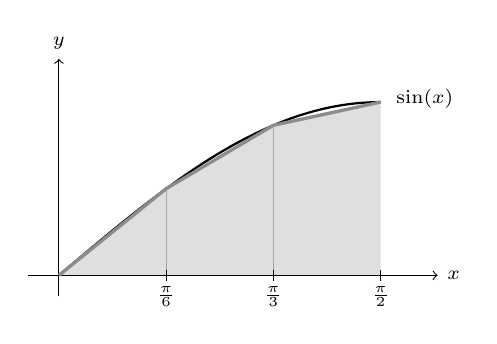
\begin{tikzpicture}[xscale=2.6,yscale=2.2]
			\foreach \l/\r in {0/0.5236,0.5236/1.0472,1.0472/1.5708}{
				\fill[gray!25] ({\l},0) -- ({\l},{sin(\l r)}) -- ({\r},{sin(\r r)}) -- ({\r},0) -- cycle;
				\draw[gray!70] ({\l},0) -- ({\l},{sin(\l r)});
			}
			\draw[->] (-0.15,0) -- (1.85,0) node[right] {\scriptsize $x$};
			\draw[->] (0,-0.12) -- (0,1.25) node[above] {\scriptsize $y$};
			\draw[thick,domain=0:1.5708,samples=80,smooth] plot ({\x},{sin(\x r)});
			\draw[very thick,gray!90] (0,0) -- (0.5236,0.5) -- (1.0472,0.8660) -- (1.5708,1);
			\draw (1.5708,0.03) -- (1.5708,-0.03); \node[below] at (1.5708,-0.01) {\scriptsize $\frac{\pi}{2}$};
			\draw (0.5236,0.03) -- (0.5236,-0.03); \node[below] at (0.5236,-0.01) {\scriptsize $\frac{\pi}{6}$};
			\draw (1.0472,0.03) -- (1.0472,-0.03); \node[below] at (1.0472,-0.01) {\scriptsize $\frac{\pi}{3}$};
			\node[right] at (1.60,1.02) {\scriptsize $\sin(x)$};
		\end{tikzpicture}
	\end{center}
	The three trapezoids are bounded above by \textit{chords} of the curve.
	Since $\sin$ is concave here, every chord lies \textit{below} the arc it subtends, so the shaded area misses a small sliver under each arc.

	The approximation is an \textit{under}-estimate, which is expected: $\sin$ is concave on $[0,\pi/2]$, so every chord lies below the curve.

	\paragraph{Exercise $\delta$:} Simpson's rule, $n = 2$, for $\displaystyle \int_0^{\pi/2}\sin(x)\,dx$

	Simpson's rule replaces the curve by a \textit{parabola} through three consecutive nodes:
	$$
	\int_a^b f(x)\,dx \approx \frac{h}{3}\left[ f(x_0) + 4f(x_1) + f(x_2) \right],
	\qquad h = \frac{b-a}{n} = \frac{\pi/2}{2} = \frac{\pi}{4}
	$$
	The nodes are $0, \frac{\pi}{4}, \frac{\pi}{2}$, and
	$$
	\int_0^{\pi/2}\sin(x)\,dx
	\approx \frac{\pi}{12}\left[ \sin(0) + 4\sin\left(\frac{\pi}{4}\right) + \sin\left(\frac{\pi}{2}\right) \right]
	= \frac{\pi}{12}\left[ 0 + 4\cdot\frac{\sqrt{2}}{2} + 1 \right]
	= \frac{\pi}{12}\left( 2\sqrt{2} + 1 \right)
	$$
	$$
	\approx 0.2618 \times 3.8284 \approx 1.002
	$$
	The error is now about $0.23\%$ --- ten times better than the trapezoidal rule with \textit{more} nodes.
	\begin{center}
		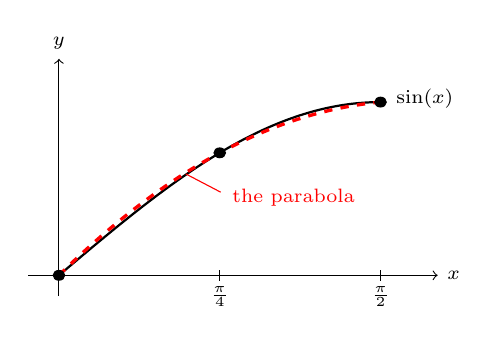
\begin{tikzpicture}[xscale=2.6,yscale=2.2]
			\draw[->] (-0.15,0) -- (1.85,0) node[right] {\scriptsize $x$};
			\draw[->] (0,-0.12) -- (0,1.25) node[above] {\scriptsize $y$};
			\draw[thick,domain=0:1.5708,samples=80,smooth] plot ({\x},{sin(\x r)});
			\draw[very thick,red,dashed,domain=0:1.5708,samples=60,smooth] plot ({\x},{-0.3358*\x*\x+1.16407*\x});
			\filldraw (0,0) circle (0.8pt);
			\filldraw (0.7854,0.7071) circle (0.8pt);
			\filldraw (1.5708,1) circle (0.8pt);
			\draw (0.7854,0.03) -- (0.7854,-0.03); \node[below] at (0.7854,-0.01) {\scriptsize $\frac{\pi}{4}$};
			\draw (1.5708,0.03) -- (1.5708,-0.03); \node[below] at (1.5708,-0.01) {\scriptsize $\frac{\pi}{2}$};
			\node[right] at (1.60,1.02) {\scriptsize $\sin(x)$};
			\node[red,right] at (0.80,0.45) {\scriptsize the parabola};
			\draw[red] (0.79,0.48) -- (0.62,0.585);
		\end{tikzpicture}
	\end{center}
	The dashed parabola through the three nodes is almost indistinguishable from $\sin$ on this interval --- which is why three nodes here beat the four nodes of the trapezoidal rule.

	A parabola simply fits a smooth curve much better than a straight line does.


	\section{Applications}

	\paragraph{Areas between curves}\mbox{}\\
	The two curves $y = \sin(x)$ and $y = -\sin(x)$ meet where $\sin(x) = -\sin(x)$, i.e. $\sin(x) = 0$, which on $[0,\pi]$ happens at $x = 0$ and $x = \pi$ --- the two ends of the interval.
	Between them $\sin(x) \geq 0$, so $\sin(x)$ is the upper curve and $-\sin(x)$ the lower one.

	The area between two curves is the integral of (upper $-$ lower):
	$$
	\mathcal{A} = \int_0^{\pi} \Big( \sin(x) - \left(-\sin(x)\right) \Big) dx
	= 2\int_0^{\pi} \sin(x)\,dx
	= 2\Big[ -\cos(x) \Big]_0^{\pi}
	= 2\Big( \underbrace{-\cos(\pi)}_{=\,1} + \underbrace{\cos(0)}_{=\,1} \Big) = 4
	$$

	\begin{center}
		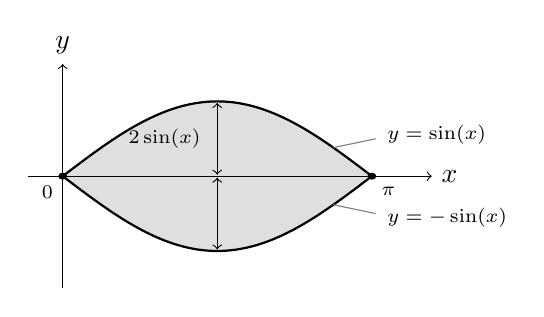
\begin{tikzpicture}[xscale=1.25,yscale=0.95]
			\fill[gray!25] plot[domain=0:pi,samples=100,smooth] (\x,{sin(\x r)}) -- plot[domain=pi:0,samples=100,smooth] (\x,{-sin(\x r)}) -- cycle;
			\draw[->] (-0.35,0) -- (3.75,0) node[right] {$x$};
			\draw[->] (0,-1.5) -- (0,1.5) node[above] {$y$};
			\draw[thick,domain=0:pi,samples=100,smooth] plot (\x,{sin(\x r)});
			\draw[thick,domain=0:pi,samples=100,smooth] plot (\x,{-sin(\x r)});
			\filldraw (0,0) circle (1.1pt); \filldraw (pi,0) circle (1.1pt);
			\node[below left] at (0,0) {\scriptsize $0$};
			\node[below right] at (pi,-0.02) {\scriptsize $\pi$};
			\node[right] at (3.2,0.55) {\scriptsize $y=\sin(x)$};
			\node[right] at (3.2,-0.55) {\scriptsize $y=-\sin(x)$};
			\draw[gray] (3.18,0.5) -- (2.75,{sin(2.75 r)});
			\draw[gray] (3.18,-0.5) -- (2.75,{-sin(2.75 r)});
			\draw[<->] (1.57,0.02) -- (1.57,0.98);
			\node[left] at (1.5,0.5) {\scriptsize $2\sin(x)$};
			\draw[<->] (1.57,-0.02) -- (1.57,-0.98);
		\end{tikzpicture}
	\end{center}
	The two dots are the points of intersection, and the vertical double arrow is the quantity being integrated: at each $x$, the region has height $\sin(x) - (-\sin(x)) = 2\sin(x)$.

	\textbf{The area is $4$.}

	\textit{Note:} the two curves are symmetric about the $x$-axis, so we could also have computed the area under $\sin$ on $[0,\pi]$ (which is $2$) and doubled it.

	\paragraph{Volume of a solid of revolution (*)} (Disk Method)\mbox{}\\
	We revolve about the $y$-axis, so we slice \textit{horizontally}: at height $y$, the slice is a disk whose radius is the distance from the axis to the curve, i.e. the $x$ such that $y = x^2$:
	$$
	r(y) = \sqrt{y}
	$$
	Each disk has area $\pi r(y)^2$ and thickness $dy$, so
	$$
	V = \int_0^1 \pi \, r(y)^2 \, dy
	= \int_0^1 \pi \left(\sqrt{y}\right)^2 dy
	= \pi \int_0^1 y \, dy
	= \pi \left[ \frac{y^2}{2} \right]_0^1
	= \frac{\pi}{2}
	$$

	\begin{center}
		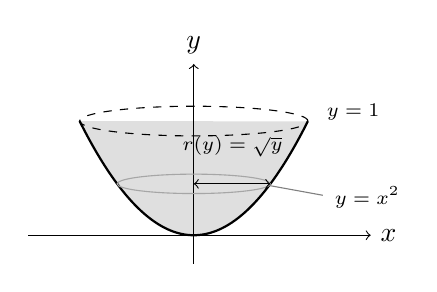
\begin{tikzpicture}[scale=1.45]
			\fill[gray!25] plot[domain=-1:1,samples=100,smooth] (\x,{\x*\x}) -- cycle;
			\draw[->] (-1.45,0) -- (1.55,0) node[right] {$x$};
			\draw[->] (0,-0.25) -- (0,1.5) node[above] {$y$};
			\draw[thick,domain=-1:1,samples=100,smooth] plot (\x,{\x*\x});
			\draw[dashed] (0,1) ellipse (1 and 0.13);
			\node[right] at (1.08,1.08) {\scriptsize $y=1$};
			\draw[gray!70] (0,0.45) ellipse (0.6708 and 0.085);
			\draw[<->] (0,0.45) -- (0.6708,0.45);
			\node[above] at (0.34,0.60) {\scriptsize $r(y)=\sqrt{y}$};
			\node[right] at (1.15,0.33) {\scriptsize $y=x^2$};
			\draw[gray] (1.13,0.35) -- (0.66,{0.66*0.66});
		\end{tikzpicture}
	\end{center}
	The grey ellipse is one of the disks being stacked: it sits at height $y$ and has radius $\sqrt{y}$.

	\textit{Sanity check:} the solid sits inside the cylinder of radius $1$ and height $1$, whose volume is $\pi \approx 3.14$; we found $\frac{\pi}{2} \approx 1.57$, comfortably smaller. \checkmark

	\paragraph{Arc length of curves}\mbox{}\\
	Here $f(x) = \frac{2}{3}x\sqrt{x} = \frac{2}{3}x^{3/2}$, so
	$$
	f'(x) = \frac{2}{3} \cdot \frac{3}{2} x^{1/2} = \sqrt{x}
	\qquad \text{and} \qquad
	1 + \left(f'(x)\right)^2 = 1 + x
	$$
	This is the point of the coefficient $\frac{2}{3}$: it makes the square root disappear from $f'$, and the quantity under the arc length root becomes simply $1+x$.
	Therefore
	$$
	L = \int_0^3 \sqrt{1+x}\;dx
	= \left[ \frac{2}{3}\left(1+x\right)^{3/2} \right]_0^3
	= \frac{2}{3}\left( 4^{3/2} - 1^{3/2} \right)
	= \frac{2}{3}\left( 8 - 1 \right)
	= \frac{14}{3} \approx 4.67
	$$

	\textit{Check the anti-derivative:} $\dfrac{d}{dx}\left[\frac{2}{3}(1+x)^{3/2}\right] = \frac{2}{3}\cdot\frac{3}{2}(1+x)^{1/2} = \sqrt{1+x}$. \checkmark

	\textit{Sanity check:} the curve joins $(0,0)$ to $\left(3, 2\sqrt{3}\right) \approx (3, 3.46)$, and the straight segment between these two points has length $\sqrt{3^2 + \left(2\sqrt{3}\right)^2} = \sqrt{21} \approx 4.58$.
	An arc is always at least as long as its chord, and $\frac{14}{3} \approx 4.67$ is indeed slightly longer. \checkmark

	\begin{center}
		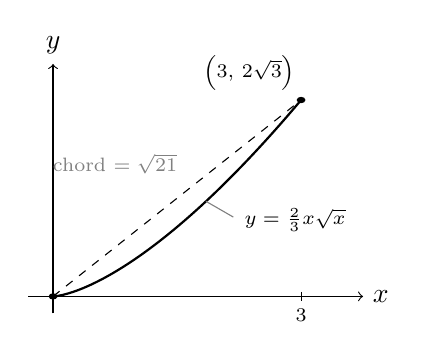
\begin{tikzpicture}[xscale=1.05,yscale=0.72]
			\draw[->] (-0.3,0) -- (3.75,0) node[right] {$x$};
			\draw[->] (0,-0.3) -- (0,4.1) node[above] {$y$};
			\draw[dashed] (0,0) -- (3,3.4641);
			\draw[thick,domain=0:3,samples=100,smooth] plot (\x,{2/3*pow(\x,1.5)});
			\filldraw (0,0) circle (1.3pt); \filldraw (3,3.4641) circle (1.3pt);
			\draw (3,0.08) -- (3,-0.08); \node[below] at (3,-0.05) {\scriptsize $3$};
			\node[above left] at (3.05,3.46) {\scriptsize $\left(3,\,2\sqrt{3}\right)$};
			\node[right] at (2.2,1.35) {\scriptsize $y=\frac{2}{3}x\sqrt{x}$};
			\draw[gray] (2.18,1.4) -- (1.85,{2/3*pow(1.85,1.5)});
			\node[gray,above left] at (1.62,1.98) {\scriptsize chord $=\sqrt{21}$};
		\end{tikzpicture}
	\end{center}
	The arc (solid) and its chord (dashed) are visibly close, which is exactly what the sanity check expressed numerically.

	\textit{Remark:} do not be fooled by how smoothly this one went.
	Arc length integrals are \textit{usually} horrible: $\sqrt{1 + (f'(x))^2}$ rarely has an elementary anti-derivative --- already for the parabola $f(x) = x^2$ it does not.
	The exercises that can be done by hand are precisely those where $1 + (f')^2$ happens to be a perfect square or a simple power.

	\paragraph{Surface area of a solid of revolution}\mbox{}\\
	We revolve the curve $y = x^2$, for $y \in [0,2]$, about the $y$-axis.

	The surface area of a solid of revolution is \textit{not} $\int 2\pi r \, dy$: a strip of the surface is slanted, so its width is the arc length element $ds$, not $dy$.
	The correct formula is
	$$
	\mathcal{A} = \int 2\pi \, r \, ds
	$$
	where $r$ is the distance to the axis of revolution.

	\begin{center}
		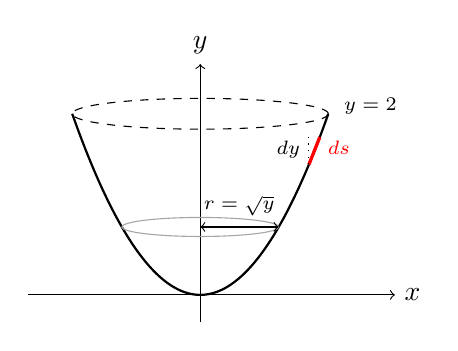
\begin{tikzpicture}[scale=1.15]
			\draw[->] (-1.9,0) -- (2.15,0) node[right] {$x$};
			\draw[->] (0,-0.3) -- (0,2.55) node[above] {$y$};
			\draw[thick,domain=-1.4142:1.4142,samples=100,smooth] plot (\x,{\x*\x});
			\draw[dashed] (0,2) ellipse (1.4142 and 0.17);
			\node[right] at (1.48,2.08) {\scriptsize $y=2$};
			\draw[gray!70] (0,0.75) ellipse (0.866 and 0.105);
			\draw[<->] (0,0.75) -- (0.866,0.75);
			\node[above] at (0.43,0.76) {\scriptsize $r=\sqrt{y}$};
			\draw[very thick,red] (1.2,1.44) -- (1.32,1.7424);
			\node[red,right] at (1.30,1.62) {\scriptsize $ds$};
			\draw[dotted] (1.2,1.44) -- (1.2,1.7424);
			\node[left] at (1.21,1.60) {\scriptsize $dy$};
		\end{tikzpicture}
	\end{center}
	The picture shows why: the strip of surface (in red) follows the \textit{slant} of the curve, so it is longer than the vertical rise $dy$ (dotted).

	Since we revolve about the $y$-axis, it is easiest to integrate with respect to $y$.
	On the curve, $x = \sqrt{y}$, so the radius is $r = \sqrt{y}$, and
	$$
	\frac{dx}{dy} = \frac{1}{2\sqrt{y}}
	\qquad \Longrightarrow \qquad
	ds = \sqrt{1 + \left(\frac{dx}{dy}\right)^2}\;dy = \sqrt{1 + \frac{1}{4y}}\;dy = \sqrt{\frac{4y+1}{4y}}\;dy = \frac{\sqrt{4y+1}}{2\sqrt{y}}\;dy
	$$
	The two $\sqrt{y}$ now cancel, which is what makes this computation short:
	$$
	2\pi \, r \, ds = 2\pi \sqrt{y} \cdot \frac{\sqrt{4y+1}}{2\sqrt{y}}\;dy = \pi\sqrt{4y+1}\;dy
	$$
	so
	$$
	\mathcal{A} = \pi \int_0^2 \sqrt{4y+1}\;dy
	= \pi \left[ \frac{1}{6}\left(4y+1\right)^{3/2} \right]_0^2
	= \frac{\pi}{6}\left( 9^{3/2} - 1 \right)
	= \frac{\pi}{6}\left( 27 - 1 \right)
	= \frac{13\pi}{3} \approx 13.61
	$$

	\textit{Check the anti-derivative:} $\dfrac{d}{dy}\left[\frac{1}{6}(4y+1)^{3/2}\right] = \frac{1}{6}\cdot\frac{3}{2}\cdot 4 \cdot (4y+1)^{1/2} = \sqrt{4y+1}$. \checkmark

	\textit{Cross-check, integrating in $x$ instead:} the interval $y \in [0,2]$ corresponds to $x \in \left[0,\sqrt{2}\right]$, the radius is $r = x$ and $ds = \sqrt{1+4x^2}\,dx$, so
	$$
	\mathcal{A} = \int_0^{\sqrt{2}} 2\pi x \sqrt{1+4x^2}\;dx
	= 2\pi \int_1^{9} \sqrt{w}\;\frac{dw}{8}
	= \frac{\pi}{4}\left[ \frac{2}{3}w^{3/2} \right]_1^{9}
	= \frac{\pi}{6}\left(27 - 1\right)
	= \frac{13\pi}{3} \ \checkmark
	$$
	(with $w = 1+4x^2$, $dw = 8x\,dx$).
	Same answer, as it must be --- but notice how much more pleasant the $y$ version was.

\end{document}
